\newpage
\subsection{Implementing FastCards}
\visHeader
\hypertarget{fastCard vis}{}

\begin{itemize}

\item[$\blacktriangleright$] To introduce fast cards into your learning box, return to the metamodel and create a new \texttt{eclass}, \texttt{FastCard}.
Quick-link to \texttt{Card} and choose \texttt{Create Inheritance} from the context menu. You don't need to override anything, so
when the \texttt{Overrides \& Implementations} dialogue appears, make sure nothing is selected. Your metamodel should now resemble
Fig.~\ref{fig:metamodel_FastCard}.

\vspace{0.5cm}

\begin{figure}[htp]
\begin{center}
  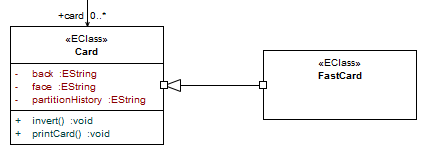
\includegraphics[width=0.9\textwidth]{ea_EClassFastCard}
  \caption{Fast cards are a special kind of card}  
  \label{fig:metamodel_FastCard}
\end{center}
\end{figure}

\vspace{0.5cm}

\item[$\blacktriangleright$] Now return to the \texttt{check} SDM (in \texttt{Partition}) and extend the control flow as depicted in
Fig.~\ref{fig:extendCheck}.

\begin{figure}[htbp]
\begin{center}
  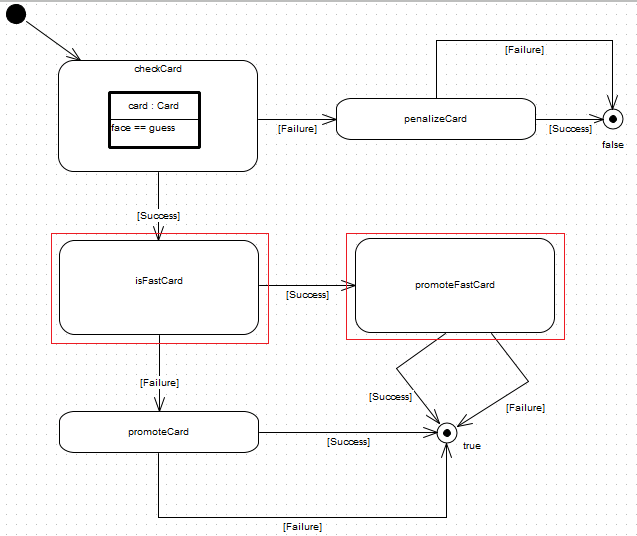
\includegraphics[width=\textwidth]{ea_extendCheck}
  \caption{Extend check to handle fast cards.}  
  \label{fig:extendCheck}
\end{center}
\end{figure}
 
 \vspace{0.5cm}
 
\item[$\blacktriangleright$] As you can see, you have created two new story nodes, the \texttt{isFastCard} assertion, and the \texttt{promoteFastCard} movement.

\vspace{0.5cm}
 
\item[$\blacktriangleright$] Next, in order to complete the newest conditional, create a bound \texttt{fastcard} object in \texttt{isFastCard}. 

\vspace{0.5cm}
 
\item[$\blacktriangleright$] To check the dynamic type, we'll need to create a binding of \texttt{card} (of type \texttt{Card}) to \texttt{fastcard} (of
type \texttt{FastCard}), so edit the \texttt{Binding} tab in the \texttt{Object Variable Properties} dialogue (Fig.~\ref{fig:fastCardBinding}). As you can see,
this set-up configures the pattern matcher to check for types, rather than \texttt{parameters} and \texttt{attributes} as we've previously encountered.
  
\begin{figure}[htbp]
\begin{center}
  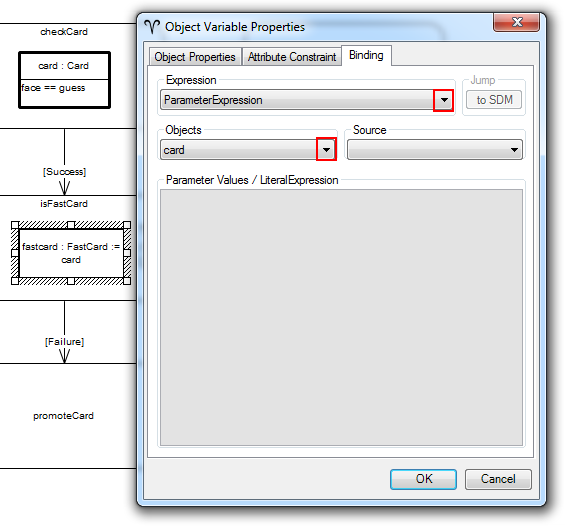
\includegraphics[width=0.9\textwidth]{ea_fastCardBinding}
  \caption{Create a binding for \texttt{fastcard}}  
  \label{fig:fastCardBinding}
\end{center}
\end{figure}

 \clearpage

In our case, we could use a ParameterExpression or an ObjectVariableExpression as \texttt{card} is indeed a parameter \emph{and} has already been used in
\texttt{checkIfGuessIsCorrect}. 

\vspace{0.5cm}

\item[$\blacktriangleright$] Since we haven't used \texttt{ObjectVariableExpression} before, lets update our \texttt{fastcard} binding to try it out! Switch
the expression to \texttt{Object\-Vari\-able\-Ex\-pres\-sion} with \texttt{card} as the target. 

\clearpage

\item[$\blacktriangleright$] To finalize the SDM, extract the \texttt{promoteFastCard} story pattern and build the pattern according to
Fig.~\ref{fig:promoteFastCardPattern}. Compare this pattern to Figs.~\ref{fig:sdm_check_complete_activity_node} and \ref{fig:sdm_check_complete_penalize}, the
original promotion and penalising card movements. As you can see, they're very similar, except \texttt{fastCard} is transferred from the current partition
(\texttt{this}) immediately to the last partition in \texttt{box}, identified as having no \texttt{nextPartition} with an appropriate NAC.

\vspace{0.5cm}

\begin{figure}[htbp]
\begin{center}
  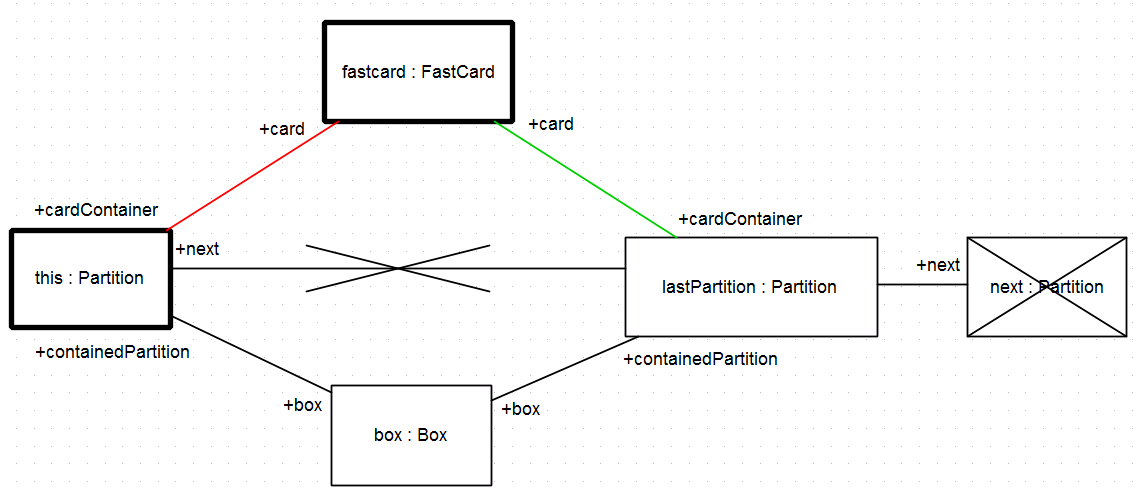
\includegraphics[width=\textwidth]{ea_promoteFastCardPattern}
  \caption{Story pattern for handling fast cards.}  
  \label{fig:promoteFastCardPattern}
\end{center}
\end{figure}

\vspace{0.5cm}

\item[$\blacktriangleright$] Inspect Fig.~\ref{fig:promoFastCardFinal} to see how this is finalized in the textual syntax.

\item[$\blacktriangleright$] You have now implemented every method using SDMs - fantastic work! Validate, export, and build
to generate the new code for your metamodel. Inspect the implementation for \texttt{check}.  Can you find the generated type casts for \texttt{fastcard}?

\item[$\blacktriangleright$] At this point, we encourage you to read each of the textual SDM instructions to try and understand the full scope of eMoflon's
features (which start on page~\hyperlink{page.9}{9}) but you are of course, free to carry on.

\jumpSingle{sec:conbran}

\end{itemize}
